Предположим, что параметр $\theta$ известен, тогда управление может быть легко найдено, как:

\begin{equation}
    u = -\theta x - \lambda x + \lambda g
    \label{control}
\end{equation}

Проведем моделирование полученной замкнутой системы в условиях скачкообразного трехкратного увеличения параметра $\theta$, получим следующие графики:

\begin{figure}
    \centerline{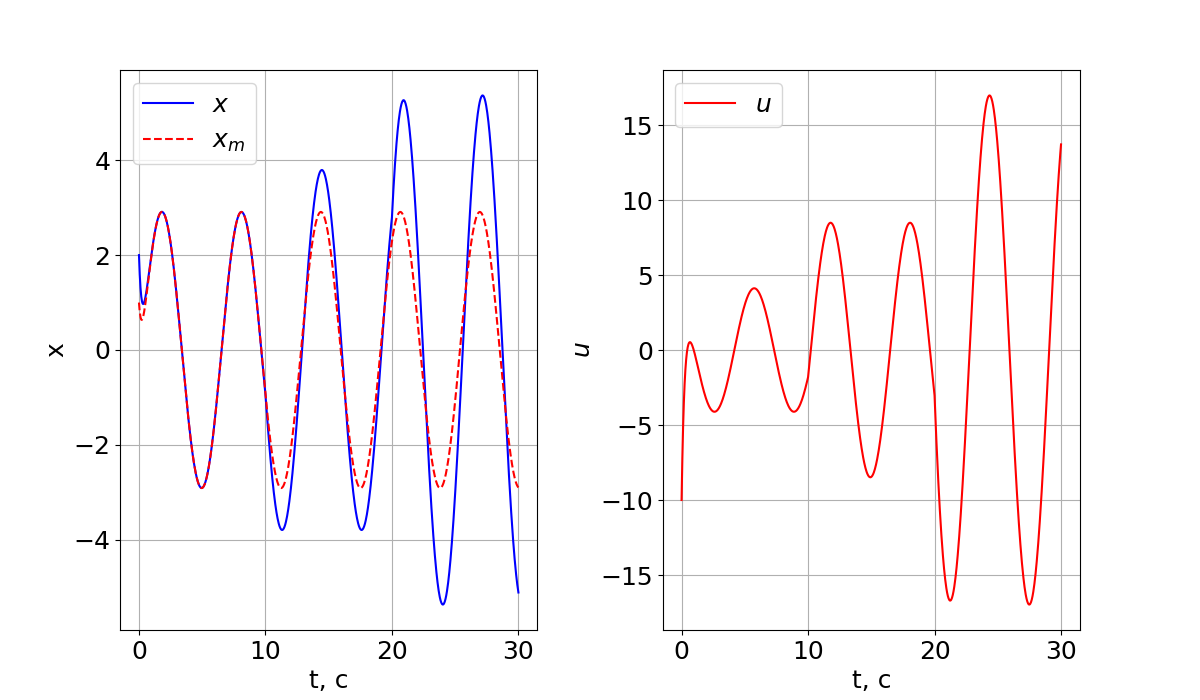
\includegraphics[width=\linewidth]{images/task_1.png}}
    \caption{График переходного процесса и управляющего воздействия для неадаптивной системы}
    \label{10}
\end{figure}

Как можно видеть, замкнутая система идеально следит за сигналом.
Попробуем теперь промоделировать таким образом, чтобы регулятор не знал об изменении параметра $\theta$ (то есть регулятор считает, что $\theta$ - известная константа)

\begin{figure}
    \centerline{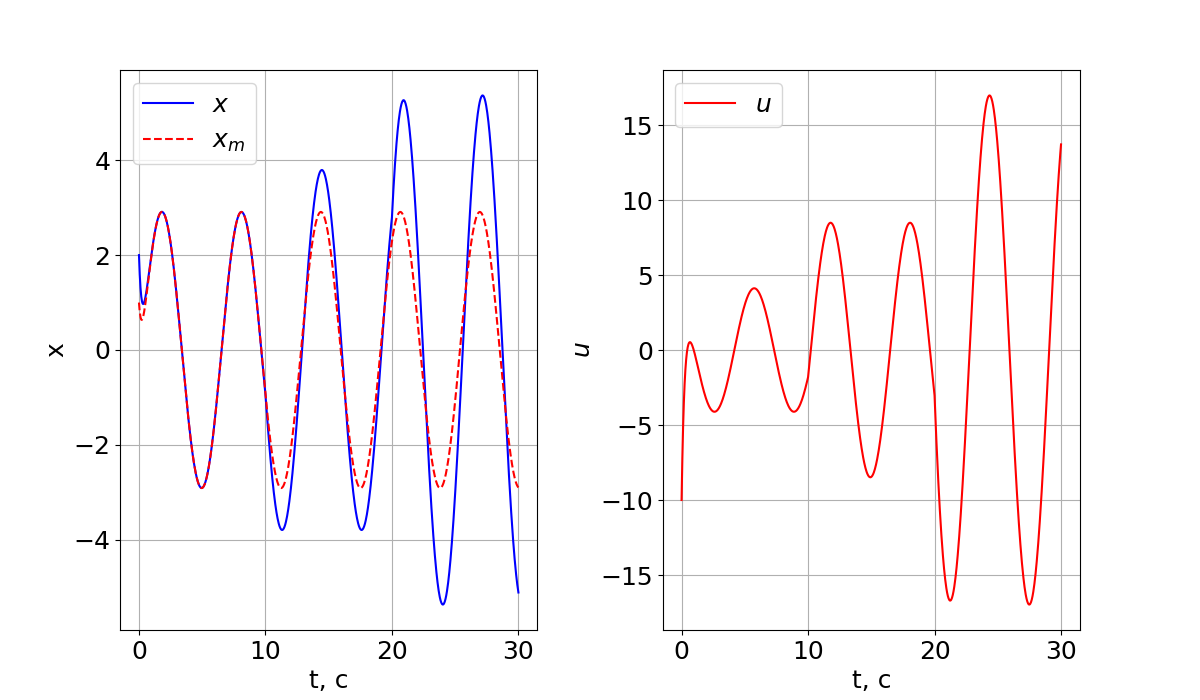
\includegraphics[width=\linewidth]{images/task_1_2.png}}
    \caption{График переходного процесса и управляющего воздействия для неадаптивной системы, при константном параметре $\theta$ при расчете управления}
    \label{11}
\end{figure}

До изменения параметра $\theta$ система идеально следила за эталонным сигналом, но после изменения, логичным образом, наблюдаем как система совершенно не справляется с задачей.

